\providecommand{\WalletOverviewFigure}{
	\begin{figure}[htbp]
		\centering
		\begin{tikzpicture}[
			node distance=1.2cm and 1.6cm,
			every node/.style={font=\footnotesize\ttfamily},
			align=center,
			box/.style={draw, minimum width=4.2cm, minimum height=3.6cm}
			]
			
			\node[box] (wallet1) {
				Wallet 1\\[0.3cm]
				Secret key:\\
				0245a349...6130\\[0.3cm]
				Public key:\\
				0357048e...ce2b
			};
			
			\node[box, right=of wallet1] (wallet2) {
				Wallet 2\\[0.3cm]
				Secret key:\\
				df60ed2d...f9bb\\[0.3cm]
				Public key X:\\
				d50cf8d1...ed45\\[0.3cm]
				Public key Y:\\
				71bf8c8b...e08e
			};
			
			\node[box, right=of wallet2] (wallet3) {
				Wallet 3\\[0.3cm]
				Secret key:\\
				8c10c0c2...42e6\\[0.3cm]
				Public key:\\
				037f9449...a3abc
			};
			
			\node[below=2.6cm of wallet1] (addr1) {\shortstack{Address (BTC)\\16tay2XDBFSV3tBpTNfHCyRAt\\WarT1hWdE}};
			\node[below=2.6cm of wallet2] (addr2) {\shortstack{Address (ETH)\\0x35a53747aba81a63\\579b6c534d16db98\\1d677889}};
			\node[below=2.6cm of wallet3] (addr3) {\shortstack{Address (BTC)\\18kh6FQB7QwC9NBynN7pNWhe\\b6CmsDNSdR}};
			
			\draw[->] (wallet1.south) -- node[right, yshift=-4pt] {\scriptsize Derivation} (addr1.north);
			\draw[->] (wallet2.south) -- node[right, yshift=-4pt] {\scriptsize Derivation} (addr2.north);
			\draw[->] (wallet3.south) -- node[right, yshift=-4pt] {\scriptsize Derivation} (addr3.north);
			
			\node[fit=(wallet1)(wallet2), draw, dashed, label=above:{Account 1}, inner sep=0.5cm, minimum height=5.1cm] (acc1) {};
			\node[fit=(wallet3), draw, dashed, label=above:{Account 2}, inner sep=0.5cm, minimum height=5.1cm] (acc2) {};
			
			\node[fit=(acc1)(acc2), draw, dashed, label=above:{Example identity}, inner sep=0.5cm] (identity) {};
			
		\end{tikzpicture}
		\caption{Relationship between identity, accounts, wallets, key pairs, and blockchain addresses.}
		\label{fig:wallet-overview}
	\end{figure}
}

\providecommand{\BIPWalletFigure}{
	\begin{figure}[htbp]
		\centering
		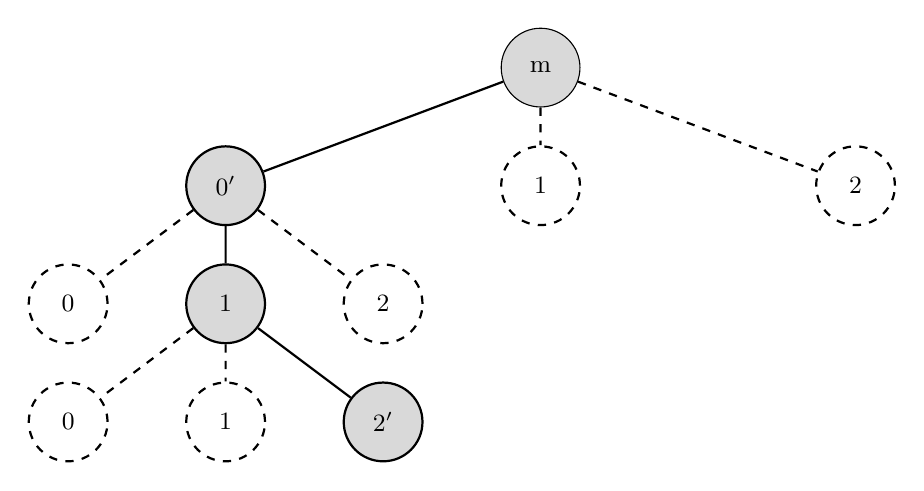
\begin{tikzpicture}[
			level 1/.style={sibling distance=4cm},
			level 2/.style={sibling distance=2cm},
			level 3/.style={sibling distance=2cm},
			every node/.style={circle, draw, minimum size=1cm, align=center, font=\small},
			selected/.style={fill=gray!30},
			dashed edge/.style={draw, thick, dashed},
			solid edge/.style={draw, thick}
			]
			
			\node[selected]{m}
			child[solid edge] {node[selected] {$0'$}
				child[dashed edge] {node {0}}
				child[solid edge] {node[selected] {1}
					child[dashed edge] {node {0}}
					child[dashed edge] {node {1}}
					child[solid edge] {node[selected] {$2'$}}
				}
				child[dashed edge] {node {2}}
			}
			child[dashed edge] {node {1}}
			child[dashed edge] {node {2}};
			
		\end{tikzpicture}
		\caption{Derivation path $m/0'/1/2'$ in a BIP32 hierarchical tree.}
		\label{fig:bip32-path}
	\end{figure}
}

\providecommand{\StatefulWalletFigure}{	
	\begin{figure}[htbp]
		\centering
		\begin{tikzpicture}[
			every node/.style={font=\sffamily\small},
			box/.style={draw, fill=gray!20, rounded corners, minimum width=1.4cm, minimum height=0.9cm, align=center},
			proc/.style={draw, rounded corners, minimum width=1.6cm, minimum height=0.9cm},
			arrow/.style={-Stealth, thick},
			]
			
			\node[proc] (keygen) at (0,0) {\texttt{KeyGen}};
			
			\node[box] (pk0) at (2.2,1.8) {pk\textsubscript{0}};
			\node[box] (sk0) at (2.2,-1.8) {sk\textsubscript{0}};
			\node[box] (st) at ($(pk0)!0.5!(sk0)$) {$st$}; % <-- Neu positioniert in der Mitte
			
			\node[box] (id) at (4.5,0) {$i$};
			
			\node[proc] (pkder) at (4.5,1.8) {\texttt{PKDer}};
			\node[proc] (skder) at (4.5,-1.8) {\texttt{SKDer}};
			
			\node[box] (pki) at (6.7,1.8) {pk\textsubscript{i}};
			\node[box] (ski) at (6.7,-1.8) {sk\textsubscript{i}};
			
			\draw[arrow] (keygen) -- (st);
			\draw[arrow] (st) -- (pk0);
			\draw[arrow] (st) -- (sk0);
			
			\draw[arrow] (pk0) -- (pkder);
			\draw[arrow] (st) -- (pkder);
			\draw[arrow] (id) -- (pkder);
			\draw[arrow] (pkder) -- (pki);
			
			\draw[arrow] (sk0) -- (skder);
			\draw[arrow] (st) -- (skder);
			\draw[arrow] (id) -- (skder);
			\draw[arrow] (skder) -- (ski);
			
		\end{tikzpicture}
		\caption{Session key derivation in a stateful wallet}
		\label{fig:stateful-wallet}
	\end{figure}
}
